\documentclass[12pt,a4paper]{article}
\usepackage{times}
\usepackage{durhampaper}
\usepackage{harvard}


% ---------------------------------
% ---- PACKAGES -------------------
    % package to add wrapfigure
    \usepackage{wrapfig}
    % packages to add images
    \usepackage{graphicx}
    % packages for pseudocode and algorithms
    \usepackage{amsmath}
    \usepackage{algorithm}
    \usepackage[noend]{algpseudocode}
    \makeatletter
    \def\BState{\State\hskip-\ALG@thistlm}
    \makeatother
    % packages to generate neural network graph
    \usepackage{tikz}
    \usetikzlibrary{matrix,chains,positioning,decorations.pathreplacing,arrows}
    % package to add graphs
    \usepackage{pgfplots}
    % stuff for checkerboard
    \usetikzlibrary{matrix.skeleton}
    \tikzstyle{ball} = [circle, shading=ball, minimum size=1cm]
    \newcommand{\bl}{\node [ball, ball color=black!80!white, draw=black!65!white, thin]{};}
    \newcommand{\wh}{\node [ball, ball color=white] {};}
% ---- END PACKAGES ---------------
% ---------------------------------

\citationmode{abbr}
\bibliographystyle{agsm}
% Titular Information
\title{A Neuroevolutionary Approach to Draughts Playing Agents}
\author{}
\student{T. P. Nguyen}
\supervisor{S. Dantchev}
\degree{BSc Computer Science}
\date{}

% Start the Document
% Note that the whole report, including the references, should not be longer than 20 pages in length.  The system will not accept any report longer than 20 pages.  It should be noted that not all the details of the work carried out in the project can be represented in 20 pages.  It is therefore vital that the Project Log book be kept up to date as this will be used as supplementary material when the project paper is marked.  There should be between 10 and 20 referenced papers---references to Web based pages should be less than 10\%.
\begin{document}
\maketitle
% Doneish (WAIT FOR CONCLUSION)


\begin{abstract}
    % These instructions give you guidelines for preparing the final paper.  DO NOT change any settings, such as margins and font sizes.  Just use this as a template and modify the contents into your final paper.  Do not cite references in the abstract.

    % The abstract must be a Structured Abstract with the headings {\bf Context/Background}, {\bf Aims}, {\bf Method}, {\bf Results}, and {\bf Conclusions}.  This section should not be longer than half of a page, and having no more than one or two sentences under each heading is advised.

    {\bf Background}

    Presently, competitive Draughts AI players are currently designed to play at a fixed ability. While it has produced very competitive and intelligent players, they require some human intervention to improve their performance. 
    This is due to their dependency on pre-defined move databases. Optimal moves are pre-calculated, and recalled when necessary. Through neuroevolution, this issue could possibly be solved by creating a player that can grow in ability over time, by learning to play itself.
    
    {\bf Aims}

    The purpose of this project is to explore an neuroevolutionary approach to tackle the game of English Draughts. First, we study previous historical successes in the field, and look at the components that helped build their systems. Then, we look at how they can be adapted to suit the objective at hand. The project will establish whether neuroevolution is a viable approach to the problem.
    
    {\bf Method}

    % The initial population consists of randomly generated AI players, which will play each other to determine the best player out of the population. The performance of championing AI players at every generation of the genetic algorithm are measured against previous champions. Appropriate algorithms are implemented to determine the overall development of the system's ability to play Draughts.

    The method starts with designing a feed-forward neural network that evaluates the advantage a particular player, given a state of a checkerboard. This is then used in a algorithm that evaluates future moves to predict the best move at a given position. This, alongside a set of weights for the neural network, creates a player that can evaluate potential moves. Finally, the player is then used on an existing Draughts framework that will provide the player with the ability to play Draughts. Genetic algorithms are used to adjust the weights of the neural network, with the intention of making the system learn to evaluate checkerboards more precisely.

    {\bf Results}

    % Using a non-trivial set of face images (i.e. with variation in face characteristics and orientation), maximum accuracy rates are 98.08% for face detection, 94.81% for face identification, however the solution could not solve the gender classification problem on this set of images. The only accuracy gained for use of an ensemble was for face detection, with a gain of 0.25% over a single neural network. The solution was very robust to image blur, and somewhat robust to image noise.

    The system has shown to perform considerably without any training, and has shown to improve over time. However, the system is not necessarily the most efficent of methods. 

    {\bf Conclusion}

    % The solution is very appropriate for the problems of face detection and face identification, but inappropriate for gender classification. Neural network ensembles remain of interest, but a simple ensemble of clones operating with ‘bagging’ training method and majority vote system did not produce satisfactory accuracy gains. The robustness of the solution to poor-quality images is indicative of its practical worth.

    The solution is very appropiate for games that do not involve the use of training data.
    When using genetic algorithms with feed-forward neural networks, it 
    The robustness of the system is quite volatile, and is best paired with mutation methods that are not heavily reliant on entropy.

\end{abstract}
% Done
\begin{keywords}
    Artificial Intelligence, Neural Networks, Genetic Algorithms, Draughts, Machine Learning, Monte Carlo Tree Search, Neuroevolution
\end{keywords}
% DONE
\section{Introduction}
    % This section briefly introduces the general project background, the research question you are addressing, and the project objectives.  It should be between 2 to 3 pages in length.  Do not change the font sizes or line spacing in order to put in more text.
    The intention of this project is to explore the effectiveness of genetic algorithms to improve the neurons of a neural network. Neural networks can be used to evaluate the performance of two players in a zero-sum game of Draughts. We attempt to manipulate the neurons through the use of genetic algorithms to increase the accuracy of the evaluation. This would potentially allow us to create an effective Draughts playing agent that, when provided with the option to consider a set of moves, would have the ability to play and learn without human input.

    \subsection*{Draughts}

    English Draughts (or Checkers) is a popular 2-player board-game played on an 8x8 chess board. Players choose a colour and begin with 12 pawns each of their respective colours, and they are placed on the dark-coloured squares of the board. Beginning with the black pawns, each player takes a turn to move a pawn diagonally in one square. In the event that a pawn reaches the opposite side of the board from where the piece originated, it is promoted to a king. Kings have the ability to traverse backwards in the same diagonal motion as pawns. Assuming that there is space upon landing, A piece (pawn or king) also has the option to capture their opponents piece by moving two consecutive diagonal squares, where the opponents piece is situated immediately opposing the players piece. Pieces can be captured consecutively in a single turn if the moves afford the scenario. A player wins by capturing all of their opponents pieces. A player loses by having all of their pieces captured. A draw occurs when both players agree to draw after a three-fold repetition (where both players take three moves to simulate the same position), or a player has pieces on the board but cannot move any of them. A draw can be forced when both players fail to capture a piece after a set amount of moves.

    \subsection*{Neural Networks}

    Neural Networks are non-linear statistical data-modelling tools, linking inputs and outputs adaptively in a learning process similar to how the human brain operates. Networks consist of units, described as neurons, and are joined by a set of rules and weights. The units are defined with characteristics, and appear in layers. The first layer is defined as the input layer, and the last layer being the output. Layers between the two aforementioned are described as hidden layers. Data is analysed through their propagation through the layers of neurons, where each neuron influences the content of the data as they pass through. Learning takes place in the form of the manipulation of the weights connecting the units in the layers. This allows it to model complex relationships between inputs and output, and it can also find patterns in the data. 

 	\subsection*{Genetic Algorithms}

    As subset of evolutionary algorithms in general, Genetic algorithms (GAs) are a group of search techniques used to find exact or approximate solutions to optimisation and search problems. The methodology is inspired by Charles Darwin's evolutionism theory; individuals are created by the crossover of the genetic information (genome) of their parents. Genomes are metaphors of genetic information; it typically refers to a data structure, most commonly an 1D array. Genetic Algorithms generally consist of a population of agents, a tournament selection process, algorithmic crossover mechanisms against the genomes of the agents, and the introduction of probabilistic mutation on genomes. The combination of evolutionary algorithms to train neural networks is described as Neuroevolution.

    \subsection*{Aims}

    % Research Question
    Whilst the use of evolutionary algorithms and neural networks have been explored to create draughts players, my intention is to explore the effectiveness of genetic algorithms and neural networks. The intention is to determine the possibility of developing a performing draughts playing agent by the use of Genetic Algorithms and Neural Networks.

    \subsubsection*{Minimum Objective}
        % The minimum objective of this project was to design and build a programme that would display a polygonal mesh of triangles, with help of a mesh data structure. The basic mesh data structure would have to enable future features that the next objectives would require.
        The minimum objective is to implement a feed-forward neural network, alongside a Draughts game interface for the network to evaluate on. This will need to be paired with some decision making program that will determine the move to choose at a given state of the game. Finally, a simple genetic algorithm would also need to be implemented that interacts with the neural network.

    \subsubsection*{Intermediate Objective}
        % The intermediate objective of this project was to create and incorporate the algorithms for the calculation of triangle surface normals, vertex normals and gradient (following our definition) in the initial programme, and enable visualisation of the “interesting” gradient changes and vertex normals on the mesh displayed by the programme.
        The intermediate objective involves the implementation of an interface to play against the end result, and to create a monte-carlo decision making algorithm, which will be used by the agents to evaluate better quality moves. Also, as the genetic algorithm includes a tournament mechanism which will play many games simultaneously, this will need to be implemented to run in parallel.
        
    \subsubsection*{Advanced Objective}
        % The advanced objective of this project was to evaluate the speed of the algorithms and compare it to the time complexity that we obtained from theoretical analysis of the algorithms. The final sections of this paper will show the results acquired and the analysis and evaluation of the work we carried out. 
        The advanced objective consists of producing a system that indicates that it is learning over time. The later sections of this paper evaluates the quality of the learning rate and other results. 
    
    % The remainder of this report will document the related work that was examined during the project, the proposed solution, the results collected, an evaluation of the results and the project, and a conclusion discussing the importance of this project and possible future work.
    To template the document, the later sections of the paper will discuss related and relevant work, the proposed solution, results and an evaluation of the project. Tha paper is then wrapped up with a conclusionary statement, discussing the implications of the project and potential future work.

% TODO
\section{Related Work}
    % This section presents a survey of existing work on the problems that this project addresses. it should be between 2 to 4 pages in length.  The rest of this section shows the formats of subsections as well as some general formatting information for tables, figures, references and equations.

    Historically, Draughts has been used as a testing ground for artificial intelligence and computional performance since the early introduction of computers. This is due to the relatively vast potential move space, making it difficult to brute-force, until recently. Schaeffer proposed a method to solve the game in 1996\cite{schaeffer_solving_1996}, and eventually proved a method to weakly-solve the game itself later on in 2007\cite{schaeffer_checkers_2007}. However, the premise of the project is not necessarily to solve the game itself, but to rather see whether genetic algorithms are still relevant.

    Research in artificial intelligence alone has been active since, targeting games with a higher move space, notably Chess and, more recently, Go. This section will summarise specific and notable techniques relevant to the discussion of the task at hand.

    % TODO: History
    \subsection{Arthur Samuel}
        In 1959, An early design of machine learning to play Draughts was devised by Arthur Samuel\cite{samuel_studies_1959}. His algorithm is based on the perpetual improvement of heuristics he devised, which act as an evaluator for a given state of the checkerboard. The evaluation function is calculated using the linear combination of his heuristics, which included various parameters of relevancy of the game. This includes the number of pawns, number of pawns positioned along the central diagonal, and so on. 

        His evolutionary strategy consisted of agents that have different coefficents for the heuristics, and new agents are formed using a successor's coefficents with subtle mutations.

        Samuel also described an early concept of Mini-Max, with Alpha Beta Pruning. The weights were then trained by the algorithm playing itself in a form of genetic programming. A later investigation by a checkers magazine evaluated Samuel's player to below Class B \cite{schaeffer_one_1997,fogel_evolving_2000} where Class B being categorised with an ELO range of [1600-1799]. 

        However, the work described was naturally also dependent on a set of heuristics Samuel devised. This could handicap the agent's ability to play, as they are constrained on the quality of Samuel's heuristics. 

    % TODO: Minimax Algorithm
    \subsection{Blondie24}

        The idea of evolving neural networks to play the game of Draughts is based on the success Chellapilla and Fogel had in evolving their own Checkers neural networks \cite{chellapilla_evolving_1999}. Their method used Samuel's system as a basis and modified it's evaluation method, using feed-forward neural networks instead of a linear combination. Their resulting player, Blondie24, was then taught to play without priori knowledge, in a similar vein, but with a higher level of competency.

        Blondie45 uses an evolutionary algorithm, using fifteen agents $i=1,\dots,15$, each of which consisted of two properties. The first property were weights of the neural network (which are initially random), with the second property being a self-adaptive parameter vector, $\tau_i$, which determined how random the mutations be when the agent $i$ evolved.
        
        In each generation, every agent plays each other in a round robin style tournament, and successors are chosen based on their performance from it. The best agents are chosen to mutate themselves to create new agents. Mutation is performed using the formula:

        $$
        \tau_i(j) = \tau_i(j) \cdot e^{\mu}
        $$
        
        Where $j=1,...,N_w$ represented each weight of the neural network $w$, and $\mu$ representing a random decimal in the range of $[0-1]$. 

        However, crossover mechanisms were not considered (and is thus not classified as using genetic algorithms). Blondie24's neural network structure consists of a $\left\{ 32,40,10,1 \right\}$ set, such that the input layer consisted of 32 nodes, and a single output node. The output node consists of a classifier from [-1, 1] inclusive, representing a particular advantage for a given side of the board. One fallback that can be seen with this particular method is that spatial awareness is not considered as it takes an immediate input of the positions on the board. This makes it inherently more difficult for the neural network to generate heuristics based on spatial awareness. Relative distance between pieces are not encapsulated in a method that can be immediately interpreted by the neural network.

        Blondie24's decision making algorithm primarily revolved around a mini-max algorithm with a ply cap. This algorithm, with the state of the checkerboard as an input, expands a tree of potential moves. Each node represents a state of a checkerboard. Child nodes represent a state of the checkerboard for a given move. Child nodes can only be produced from the parent node; i.e a move from a parent node will produce a child node. 
    
%        Child nodes are expanded until some depth is reached. From here, an evaluation function is used to calculate the value of the leaf nodes at this depth. This evaluation function produces a value that indicates a players advantage in a given state. The best potential position for a given player can be deduced from the nodes at this stage, which is quantified with a value.
%    
%        The best value propagates upwards until it reaches to a child of the root node. This represents an agent's current state of the game. The use of alpha-beta pruning would help to ignore evaluating unnecessary moves, reducing the number of calculations. Once the possible moves have been considered, the best child node is chosen, representing the best move at a given position.
%    
%        There are inherent trade-offs with having a higher ply count; asymptotic complexity of mini-max is exponential; it being $O(x^y)$ for $x$ being the branching factor, and $y$ being depth. Branching factor will consist of the moves from each agent in a given game. This exponential growth is the achilles heel to the mini-max approach.

        We do not wish to repeat this work, but it is important to understand that we wish to abstract and modularise parts of the best features of this system to modify and extend them in the solution described in the paper.

        \subsection{Post Blondie24}

        Blondie24 was influential in the field of neuroevolution during its time, leading to various studies on how it evolves. A notorious example is the Al-Khateeb and Kendall series, where they explore in detail the different features that comprise Blondie24. One of their insightful studies with the Look-ahead Depth \cite{al-khateeb_effect_2012} conlcuded that having a higher ply-depth increases the overall performace of the player, and that agents trained at a higher ply performs significantly worse when playing at a lower ply.
        
        The tournament approaches \cite{al-khateeb_introducing_2009}, the value of piece differences \cite{al-khateeb_importance_2010}. 
        
        % Alternative contemporary machine learning techniques have been exercised against Draughts. Franken et al. (2003) used draughtsboards as an evaluator for their rendition of an AI through Particle Swarm Optimisations.[14] 
        Quetzalcoatl Toledo-Marin et al. (2016) performed studies on attacking strategies using the game of checkers as a reference (which however can be applied to any other zero-sum game), where they mathematically prove that for an offensive player, maximising the offensive improves their probability to win.\cite{toledo-marin_is_2016}

        % Stanford's SVM method of improving Blondie
        Cobbe, et al. improves Blondie24 by using an evaluation function that consists of Support Vector Machines, which achieves locally optimal performance in approximately a third as many generations than its typical evolution. \cite{cobbe_accelerating_nodate} 
        
    % TODO: fix writeup of everything, talk about monte-carlo
    \subsection{Neural Networks}
        % need to mention regular gradient based learning
        Lai's Giraffe \cite{lai_giraffe:_2015} program used a deep reinforcement learning technique to play Chess to an advanced level in a relatively quick time-period. Giraffe's decision function involved using Temporal Difference Learning (TD-Leaf), an improvement on MiniMax, by Baxter et al. \cite{baxter_tdleaflambda_1999} However, Giraffe has been trained on previously played games from grandmaster tournaments as a reference, and was not entirely self-taught.
        % Lai then moved on to join DeepMind, 

        % talk about monte-carlo

    % TODO: fix writeup of everything
    \subsection{Return of Genetic Algorithms}
        % Ling-Xi
        In 2017 Lingxi Xie et al. took it a step further and discussed using genetic algorithms to compute optimal deep learning structures automatically, using an image recognition dataset as the benchmark for competitiveness against the networks.\cite{xie_genetic_2017}
        % Kusiak et al. (2007) have devised the use of pure genetic algorithms as the premise to evaluate the board. [16] they describe the use of 25 heuristics that, when used in unison, can determine the evaluation of a given board. They continue to go further on and specify that various combinations of heuristics, when used in different stages of the game, prove to be the most promising of outcomes.

        Since then, there has been a non-trivial number of papers within Checkers, Genetic Algorithms and Convolutional Neural Networks. Sergei Perez (UC Irvine) describes the use of genetic algorithms to evolve weights for a convolutional neural network as a more performant alternative to back-propagation, in nearly all situations, other than when the number of generations generated for neural networks are small.[21]

        % Uber's revival of genetic algorithms and safe mutations
        Interestingly, Clune et al. on behalf of Uber Labs returned to the use of genetic algorithms as a basis to train deep convolutional networks with success. \cite{such_deep_2017} Their GA-NN system is used to play popular Atari games on the OpenAI framework, and is found to perform as well as other contemporary evolution strategies and reinforcement learning algorithms. 

        This is based on their system's ability to perform safe mutations \cite{lehman_safe_2017}, a technique that revolves around measuring the sensitivity of the network to changes with some of the weights. This allows them to evolve deep neural networks, having over 100 layers and over four million weights and biases, allowing random but safe and exploratory steps. Their safe mutation exploits the knowledge of the neural network structure, by retaining sampled experiences of the network (inputs that feed into the network and its outputs). This allows the weights to be manipulated by comparing its significance with the output, by comparing it with the sampled experiences. 

        However, they also do not consider the use of crossover techniques in their paper, but they do describe that it would very well be possible to produce a safe crossover method that can exploit the structure of the neural network, inspired by the research they've produced on safe mutations.

        Unfortunately, it is unrealistic to apply the same techniques described here into the proposed system. The machine used as the base (consisting of hundreds to thousands of cores), but a more simplistic and adapted model can be produced using similar ideas. 

% TODO: Write up everything..
\section{Solution}

    % This section presents the solutions to the problems in detail.  The design and implementation details should all be placed in this section.  You may create a number of subsections, each focussing on one issue.  

    % This section should be between 4 to 7 pages in length.
 
    %We started with an implementation of the k-means method which would later be used to evaluate and compare our algorithm with. The simulation tool was programmed in C++ using OpenGL to render large quantities of dynamic objects within the environment. We alsodesigned our architecture such that we run features of our algorithm in parallel by usingsynchronisation and multithreading.
    This section describes the build of the system in order of implementation. Implementing the checkerboard interface is not included in the discussion as it is not one of our objectives. However, the sections below are considered the interface being built prior. 

    \subsection{Neural Network}
%     \begin{wrapfigure}{r}{0.37 \textwidth}
%            % \begin{center}
%            \fontsize{8}{11}
%            % \vspace{-40pt}
%            \centering
%                \caption{The indexes of the 32 pieces of the input layer are the immediate values of the positions on the board. \label{boardarray}}
%                \vspace{5pt}
%                \begin{tikzpicture}
%                \color{white}
%                \matrix (m) [matrix of nodes, nodes in empty cells, label skeleton, nodes={minimum size = 0.4cm}] {
%                & 31 &&30&&29&&28 \\
%                27 &&26&&25&&24&&\\
%                &23&&22&&21&&20\\   
%                    19&&18&&17&&16&&\\
%                &15&&14&&13&&12\\
%                11&&10&&9&&8&&\\
%                &7&&6&&5&&4\\
%                3&&2&&1&&0\\
%                % \bl &     & \bl &     &     &     & \bl &     \\
%                %     &     &     & \bl &     &     &     &     \\
%                % \wh &     &     &     &     &     &     &     \\
%                %     &     &     & \wh &     & \wh &     & \wh \\
%                % \wh &     & \wh &     & \wh &     & \wh &     \\
%                %     & \wh &     & \wh &     & \wh &     & \wh \\
%                };
%                \foreach \row in {1, ..., 8} {
%                \foreach \col in {1, ..., 8} {
%                    \pgfmathparse{Mod(\row + \col, 2) ? "black" : "white"}
%                    \colorlet{squarebg}{\pgfmathresult}
%                    \fitandstyle[background]{(m-cell-\row-\col)}{fill = squarebg}
%                }
%                }
%                \end{tikzpicture}
%            % \end{center}
%            \vspace{-20pt}
%        \end{wrapfigure}
%        % talk about how it works
%        % talk about the preprocessing
%        
        To evaluate the board, a feed-forward multilayer perceptron style neural network will be used. The network would contain 4 layers; the input layer consists of 91 nodes, with the output node having 1. Hidden layers will have 40 and 10 nodes respectively. Figure \ref{nnmodel} shows the network in the form of a diagram.

        Common knowledge infers that a king is worth more than a pawn, but it is disputed about its precise value advantage. For the sake of simplicity, a king's piece value is to be weighted at $1.5x$ a pawn value; a value of a pawn will be $1$. 

        The input array takes in the checkerboard. The intention is to weigh the Black pawns with a value of 1, and white pawns as -1. To create the input layer, we treat the checkerboard into a 1D array, with the indexes displayed in figure \ref{boardarray}. The array is used to calculate all possible sub-squares of the checkerboard, ranging from a 3x3 kernel to a 8x8. Each sub-square is summed up to create an input node. There are consequently 91 combinations of the sub-squares, thus forming the input layer. 


        \begin{wrapfigure}{r}{0.4\textwidth}
            \centering

            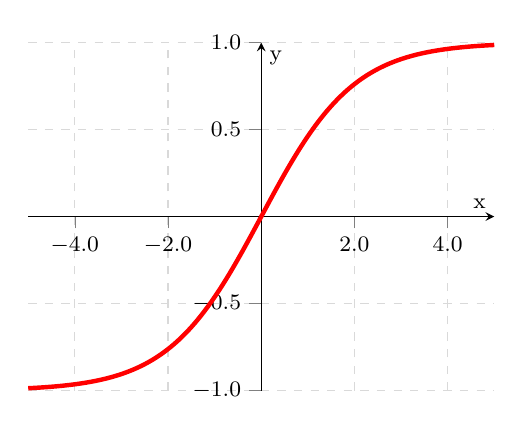
\begin{tikzpicture}
                \fontsize{8}{11}
                \begin{axis}[
                    legend pos=north west,
                    axis x line=middle,
                    axis y line=middle,
                    x tick label style={/pgf/number format/fixed,
                                        /pgf/number format/fixed zerofill,
                                        /pgf/number format/precision=1},
                    y tick label style={/pgf/number format/fixed,
                                        /pgf/number format/fixed zerofill,
                                        /pgf/number format/precision=1},
                    grid = major,
                    width=75mm,
                    height=6cm,
                    grid style={dashed, gray!30},
                    xmin=-5,     % start the diagram at this x-coordinate
                    xmax= 5,    % end   the diagram at this x-coordinate
                    ymin= -1,     % start the diagram at this y-coordinate
                    ymax= 1,   % end   the diagram at this y-coordinate
                    %axis background/.style={fill=white},
                    xlabel=x,
                    ylabel=y,
                    tick align=outside,
                    enlargelimits=false]
                % plot the stirling-formulae
                \addplot[domain=-5:5, red, ultra thick,samples=500] {2*(1/(1+e^-x))-1};
                % \addlegendentry{$f(x)=\frac{1}{1+e^{-5x}}$}
                \end{axis}
            \end{tikzpicture}
            \caption{Graph of tanh function $f(x)={\frac{2}{1+e^{-x}}- 1}$ (An example of an activation function with a sigmoid curve). \label{sigmoid}}
            \vspace{-10pt}
        \end{wrapfigure}
        
        % Talk about the activation function
        Weights of a neuron are multiplied by their input value, summed with their bias, and are passed through an activation function $O = f((Input* weight) + Bias)$ to become an input for another neuron. Activation functions, when visualised, usually have a sigmoid curve, but may also take the form of other shapes. Common characteristics of activation functions include values to be monotonically increasing, continuous, differentiable and bounded.
        % how does it work?

        Our initial choice for the activation function is tanh, shown in figure \ref{sigmoid}. There exists inherent issues related to the properties of their derivatives, discussed by Nair and Hinton \cite{nair_rectified_2010}, described as the missing gradient problem. However, since this issue is related to the properties of a gradient based learning method and not through a stochastic learning method (of which genetic algorithms are), this is not a concern for the project. Sigmoidal function also facilitates the ability to simulate a zero sum formula (for a range of -1 to 1) due to its central symmetric properties.

        Results are cached such that inputs that have been already evaluated are saved such that they can be recalled immediately. This has shown varying levels of improvement dependent on the ply depth. As the ply increases, the size of the state space increases, and therefore the chances of recalling the same set of inputs naturally decrease. This is also used for our safe mutations algorithm, described later on in 
        
    \subsection{Decision Making Algorithm}
        % talk about starting with random moves
        % talk about minimax
        % then talk about monte carlo

        The mini-max method would have a search depth of 4ply (where the agent will search four moves ahead.) This should allow the agents to form a basic strategy where they can plan their moves in advance. 

        To choose the best move given a current position, an initial decision making process for an agent revolves around the use of minimax algorithm. This was the case for Chellapilla and Fogel's agent. \cite{chellapilla_evolving_1999}. 

        \begin{figure}[!h]
            \centering
            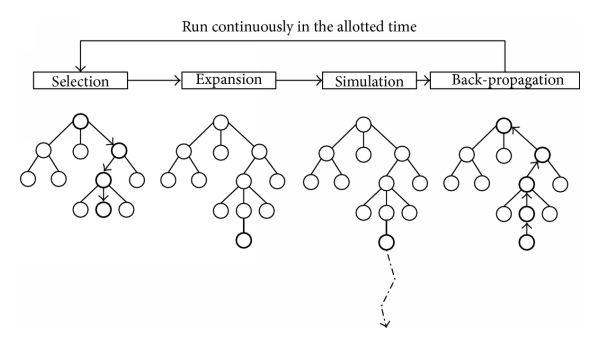
\includegraphics[width=80mm]{images/montecarlo.png}
            \caption{A diagram describing the MCTS process.}
        \end{figure}

        Once initial development on the mini-max algorithm is complete, The project would migrate to a hybrid technique that combines mini-max and a more contemporary algorithmic paradigm, Monte-Carlo Tree Search (MCTS). A basic MCTS differs from mini-max where future moves are randomly played to the end of the game. It acts as a sampling of possible outcomes, and does not depend on an evaluation function at all. The random simulation of games are skewed such that more reasonable moves are chosen. A survey by Browne et al. found that MCTS can dramatically outperform mini-max based search engines in games where evaluation functions are otherwise difficult to obtain \cite{browne_survey_2012}. MCTS are played in rounds that consist of four operations:

        \begin{itemize}
            \item Selection: A selection strategy is played recursively until some position is reached. 
            \item Play-Out: A simulated game is played. Again, a basic form of MCTS would play until an end-game is reached.
            \item Expansion: A node is added to the tree.
            \item Back-propagation: The result of the game is back-propagated in the tree of moves.
        \end{itemize}

        These rounds are repeated until a certain period of time is met or a certain number of rounds are computed. Once finished, a node is chosen based on its total probability of reaching an winning outcome.

        MCTS-EPT (or MCTS with early playout termination) is introduced by Lorentz \cite{lorentz_using_2016}. MCTS-EPT modifies the MCTS random play-out approach; Instead of allowing the random moves play to the end of the game, the number of moves traversed are capped and an evaluation function can be used from that caped position instead. The termination ply would be capped at 6ply. This could potentially improve the amount of foresight for a given set of moves, without the need to depend on random generations of moves to the end, and the need to evaluate more moves (as typically needed even with alpha-beta pruning on a mini-max algorithm).

   

        The minimax algorithm would be retained to evaluate the performance differences between the  two decision making algorithms.
        
        \begin{figure}[ht!]
            \centering
            \caption{The chosen neural network model. The preprocessed values of the checkerboard are used as input. An output is produced after propagation that ranges from [-1,1]. \label{nnmodel}}
            \vspace{10pt}
            \tikzset{%
                every neuron/.style={
                    circle,
                    draw,
                    minimum size=0.9cm
                    },
                neuron missing/.style={
                    draw=none, 
                    scale=4,
                    text height=0.333cm,
                    execute at begin node=\color{black}$\vdots$
                },
            }

            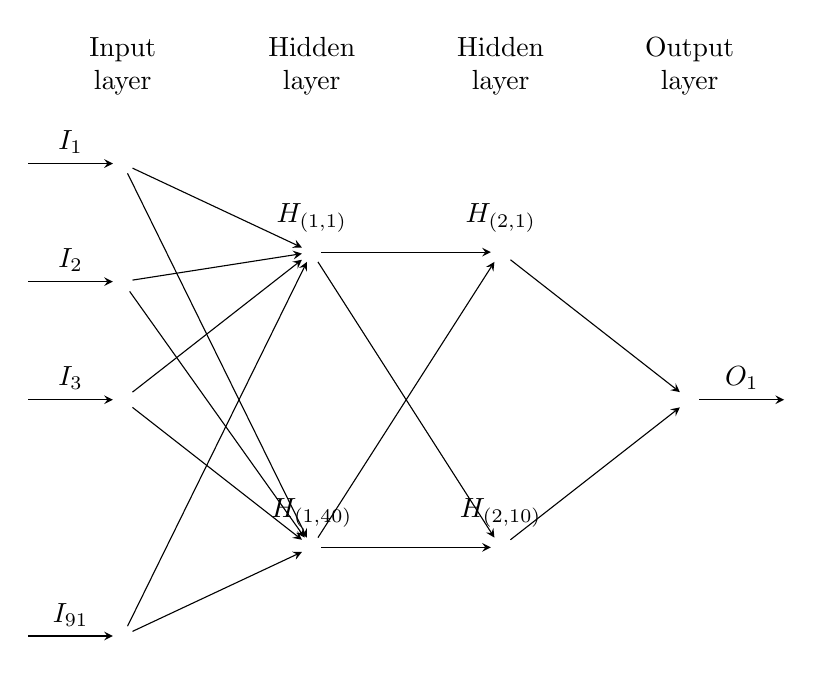
\begin{tikzpicture}[x=1.2cm, y=1.5cm, >=stealth]

            % draw nodes
                % % input values
                % \foreach \m/\l [count=\y] in {1,2,3,missing,4}
                % 	\node [every neuron/.try, neuron \m/.try] (input-\m) at (-0.5,2.5-\y) {};

                % input layer
                \foreach \m/\l [count=\y] in {1,2,3,missing,4}
                \node [every neuron/.try, neuron \m/.try] (input-\m) at (0,2.5-\y) {};
                
                % layer 1
                \foreach \m [count=\y] in {1,missing,2}
                \node [every neuron/.try, neuron \m/.try ] (hidden1-\m) at (2,2-\y*1.25) {};

                % layer 2
                \foreach \m [count=\y] in {1,missing,2}
                \node [every neuron/.try, neuron \m/.try ] (hidden2-\m) at (4,2-\y*1.25) {};

                % output layer
                \foreach \m [count=\y] in {1}
                \node [every neuron/.try, neuron \m/.try ] (output-\m) at (6,0.5-\y) {};

            % input layer
            \foreach \l [count=\i] in {1,2,3,91}
                \draw [<-] (input-\i) -- ++(-1,0)
                node [above, midway] {$I_{\l}$};

            % hidden 1
            \foreach \l [count=\i] in {{(1,1)},{(1,40)}}
                \node [above] at (hidden1-\i.north) {$H_{\l}$};

            % hidden 2
            \foreach \l [count=\i] in {(2,1),(2,10)}
                \node [above] at (hidden2-\i.north) {$H_{\l}$};

            % output layer
            \foreach \l [count=\i] in {1}
                \draw [->] (output-\i) -- ++(1,0)
                node [above, midway] {$O_\l$};

            % lines from input to hidden 1
            \foreach \i in {1,...,4}
                \foreach \j in {1,...,2}
                    \draw [->] (input-\i) -- (hidden1-\j);
            
            % lines from hidden 1 to hidden 2
            \foreach \i in {1,...,2}
            \foreach \j in {1,...,2}
                \draw [->] (hidden1-\i) -- (hidden2-\j);

            % lines from hidden 2 to output
            \foreach \i in {1,...,2}
                \foreach \j in {1}
                    \draw [->] (hidden2-\i) -- (output-\j);

            % headings
            \foreach \l [count=\x from 0] in {Input, Hidden, Hidden, Output}
                \node [align=center, above] at (\x*2,2) {\l \\ layer};

            \end{tikzpicture}
            % \vspace{-25pt}
        \end{figure}
    

    \subsection{Genetic Algorithms}
        % talk about generation of population
        % talk about tournmanent
        % talk about 
        The genetic algorithm (GA) is the premise of the system's learning strategy. GA's are used to train the neural network. We discuss the various algorithms that form the collection of GA strategies below. For the system, a population size of 15 will be chosen.

        \subsubsection{Population Generation} \label{population_generation}
            % Introduce what its for
            In genetic algorithms, the population serves as a base that allows agents in the pool to play each other. Every generation has its own population, with all having the same number of agents. The initial population will consist of randomly generated weights and biases of the neural network, with values from [-1,1]. 
            
            For a population size of 15, the next generation is created using the best five agents from the current generation. This is discussed in {\it{\ref{tournament_selection} Tournament Selection}}. 
            They will continue to play in the next generation; this strategy is described as elitism. These agents are also used as a base to create 10 new agents from. 
            
            The next eight players are generated through the use of crossover strategies, explained in {\it{\ref{crossover_strategy} Crossover Strategy}}. The weights of the $1^{st}$ and $2^{nd}$ place agents are used as input to the crossover strategy and will generate 4 offsprings. Two are reciprocal crossover representations from each other, and the other two being directly mutated from the parents themselves. Another four children will be created using the same strategy, with the 2nd and 3rd agent's weights. The remaining two will be direct mutations of the 4th and 5th place agents.

        \subsubsection{Tournament Selection} \label{tournament_selection}

            To sort the quality of the players in a population, a tournament selection process is deduced. This allows us to choose the best players who will continue to play in the next generation.

            Currently, each agent in the population would play 5 games as Black, against randomly selected opponents. Each game lasts a maximum of 100 moves from both players. If a winner is not deduced at this stage, a draw is called. Draws are also called when there is a three-fold move repetition from both players. A win is worth $2$ points, a draw being none and a loss being $-1$ points. Both the agent and its opponent receives a score from the game.
            Scores are tallied up at the end of the tournament. Players are sorted by the number of points they scored. The best players would have the highest number of points.
            
            Talk about how this is running in parallel thanks to python's muiltiprocessing library'
            
        \subsubsection{Coefficient Mutation} \label{coefficient_mutation}

            To create variation between agents in preparation for the next generation, we create statistical anomalies through the use of mutations. This is used as one of the learning mechanisms that help change the decision factors of the neural network.

            Weight and biases of an agent's neural network would increment by a random value that is created using the following formula, where $WeightP$ is the current weight, $K$ represents the number of weights and biases in the neural network, and $m$ representing a random floating point in the range of [-1,1]. Equation \ref{mutation} describes the mutation formula.

            \begin{equation} \label{mutation}
                % \caption{The mutation formula. \label{mutation}}
                WeightN = WeightP + \frac{m}{\sqrt{2 * \sqrt{K} }}
            \end{equation}

            The weights, like the activation function (in \ref{sigmoid}), will have a soft maximum of [-1, 1]. This would consequently mean that the mutation is not controlled, and dependent on the number of weights in the system; The more weights in the network implies a less significant mutation.
            
             We also choose to experiment with soft mutations, inspired by Lehman et al. \cite{lehman_safe_2017} We use a subset of precalculated neural network calculations for inputs and outputs and use this as a premise to guide our mutation. The method is as follows:
             
             \begin{enumerate}
             \item With the current set of weights $w$, choose a subset of precalculated input and output tuples $\phi_{w} = (I, \lambda_{I,w})$ where $I$ represents the input values of the network, and $\lambda_{I,w}$ as the output.
             \item Generate a perbutation of the weights calculated using Equation \ref{mutation}. Call this $y$. Use $y$ as a basis of a neural network. 
              \item Using the inputs $I$ in $\phi_{w}$, calculate a new set of input and output tuples $\phi_{y} = (I, \lambda_{I,y})$.
              \item Calculate the divergence $\delta = \lambda_{I,y} /\ \lambda_{I,w}.$ 
              \item Calculate the quality of $y$ based on the number of inequalities $\delta \geq 1$.
             \item Repeat steps 2-5 some $n$ times, keeping note of the the best $y$. 
             \end{enumerate}

            The intuition behind this is that if $\phi_{w}$ is a subset of moves that led to a winning game, then the manipulation of the weights is left open as long as it can replicate the performance of winning games. One of the concerns about this approach, also mentioned during the similar works, is the efficency of the approach. % I need to make some measurements first. 
            
        \subsubsection{Crossover Strategy} \label{crossover_strategy}

                
           \begin{figure}
                \centering
                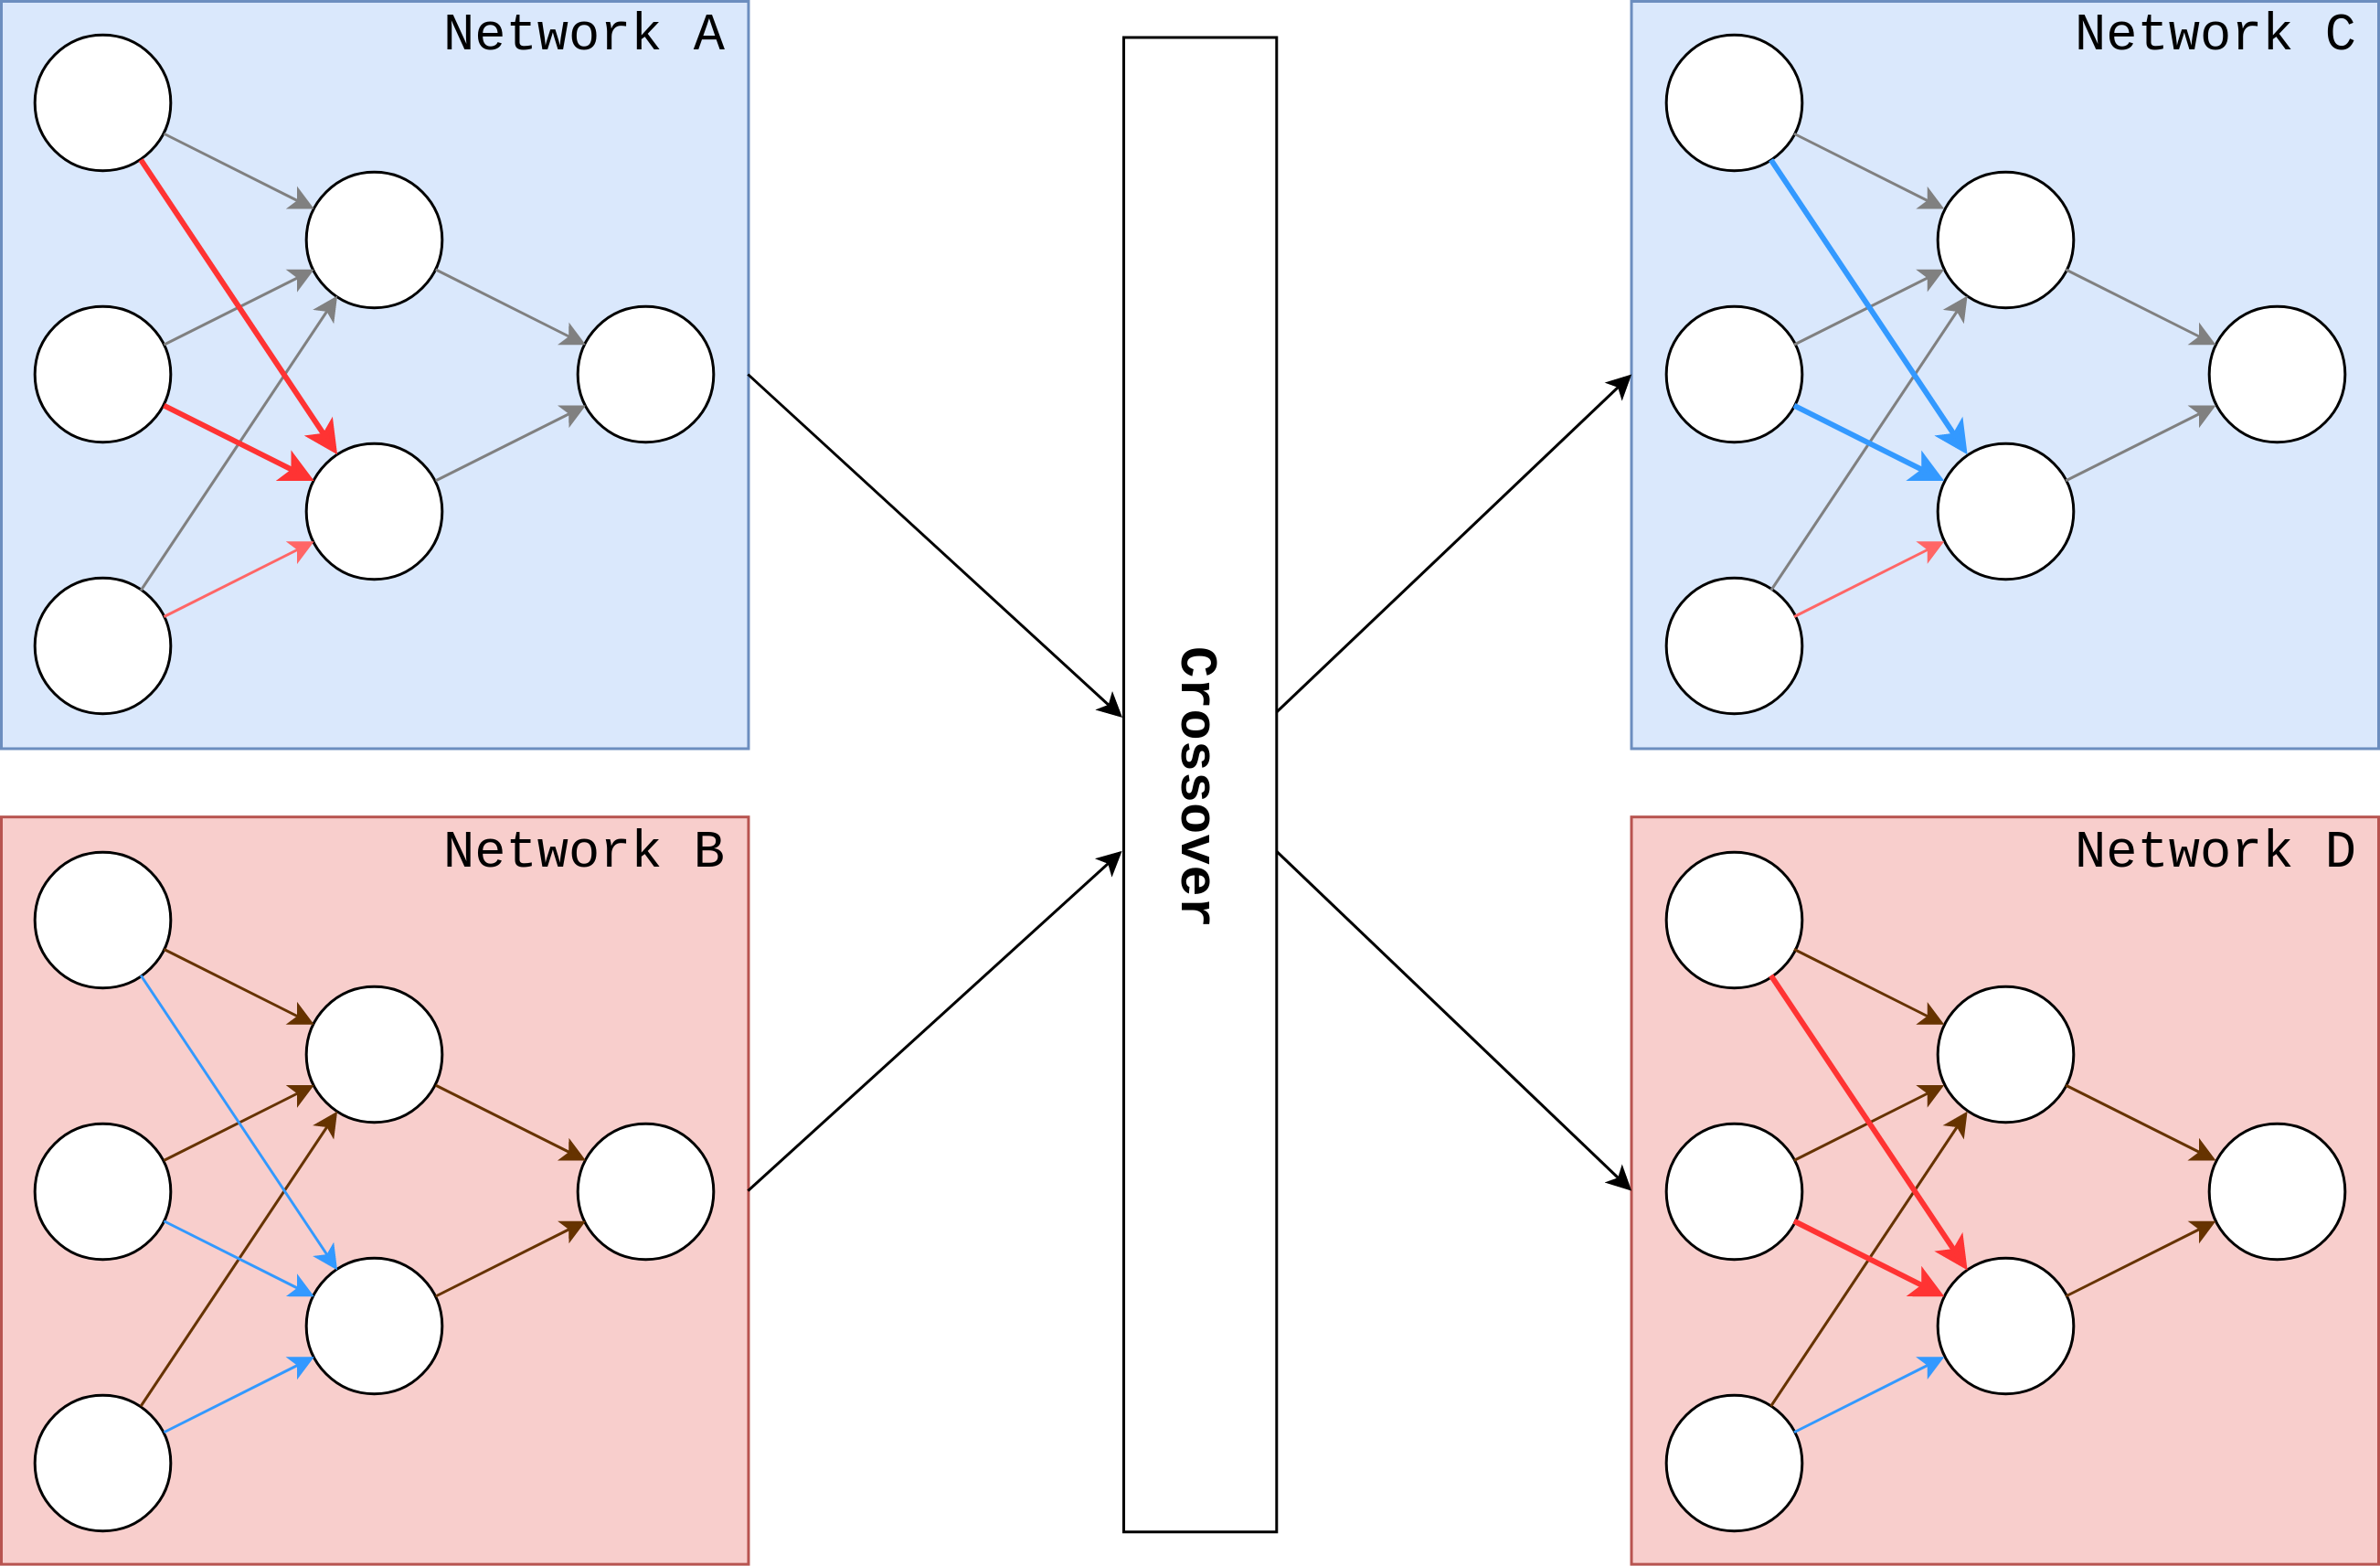
\includegraphics[width=90mm]{images/crossover.png}
                \caption{A diagram visualising the crossover process.\label{crossoverpic}}
            \end{figure}

            Another learning mechanism provided from the use of genetic algorithms is the use of crossovers. This combines the traits that build two parent agents to create children. In our scenario we use the weights and biases of the parent's neural networks.


            Two offsprings would be created from a pair of parents, with each offspring being the reciprocal crossover of each other. 
            % The weights of both parents (now each treated as a 1D array of coefficients), are divided contingent on the number of weights and biases for a given layer. Each layer should be treated separately to reduce the potential dependency on a purely randomly generated neural network. For each set of weights in a given layer, Algorithm \ref{crossover} describes the crossover process in pseudocode.
            A random node from the dominant parent's hidden nodes are chosen. A dominant parent is the agent who gained more points in the tournament round than the other (who would be the submissive parent). If a dominant parent cannot be deduced it would be randomly chosen. 


            Once a random node is chosen, The weights and biases that feed into the chosen node are swapped with the submissive parents values at the same positions. As values in the weights can range from -1 to 1, dominant input weights are values that are greater than 0.75 or less than 0.75. 
            Figure \ref{crossoverpic} shows this in more detail. In the diagram, Network A and B are parents, creating reciprocal offspring networks C and D. A is the dominant network, and A's node with the red inputs is chosen. The weights and biases of the red inputs are swapped with the values at the same position in network B. Network C is formed with Network B's dominant weights, with the rest being composed from A. Network D is the reciprocal, having Network A's dominant weights and the rest from B.

            This crossover process would create a subtle modification to a neural network, by swapping a small subset of weights and biases at a time. Having a more dramatic crossover could potentially change the structure of the network flow, reducing its effectiveness. A visualisation of the crossover process can be found in Figure \ref{crossoverpic}.
            
            % Talk about how this is not commonly used.

    \subsection{Testing}
        Initial runs will operate on a 1-ply load to determine the stability of the system on a linux (Ubuntu) machine containing a 4-core Intel i5 6600u processor with 12GB's of memory. Development and debugging will also occcur on this machine. 
        
        Once testing has proven to be stable, the system would run on Durham's MIRA distributed system (Debian) with a 6-ply move depth. This machine utilises 4 Intel Xeon E7-8860 processors (Each CPU contains 16 physical cores running in 2.2Ghz, with hyperthreading). This comes to a total of 64 Cores, and 128 threads. MIRA also comes with 256GB of DDR3 memory. 
        
        To keep simulations running on MIRA, MOSH is used to maintain a consistent connection to MIRA. The end champion is then transferred to the initial machine in order to be played against by human input. Statistical evaluations and calculations are also calculated on MIRA to reduce computational time.

        At the end of a given generation, we measure growth of performance by using the generation's champion. Presently we will use the mean of means approach. When a new champion is generated, it is played against the previous 5 champions from earlier generations. 6 games are played for each previous champion, with 3 being as Black, and 3 being White. A mean score is calculated from those 6 games. The overall performance of the current champion is the mean of the 5 sets of games. A positive improvement is when the mean of means are greater than 0. 

        Point Score for the champion games are measured by {1,0,-1} where a Win counts as 1 point and -1 for a loss. The weights are scaled differently to the regular tournament in order to accurately portray the difference between previous champions.
    
        \subsubsection*{Evaluation Method}
    
        The end player is used to create comparison games against its ancestors. This player is to be first tested against an agent who is choosing random moves, an agent who is using pure monte-carlo tree searches, and a subset of older agents prior to its current state. These statistics will be used as evidence in order to determine whether the agent is learning over time, is used as the premise to determine whether neuroevolution can be considered as a technique for non-specific domain problems.
       
    % Issues
    \subsection{Issues}
       
        - finding a computer that would run the simulations
        - appropiately saving files
        - testing neural network was difficult
        - testing move decisions were difficult
        - optimising the learning rate

    The system is implemented using Python and NumPy.
    Testing move decisions were difficult
    

    Interestingly, the machine used for training did not perform necessarily as effeciently. The system is built such that the games in the tournaments are "embarassingly parallel", but the machine does not scale accordingly. Most of the computation is spent on calculating floating point matrix operations (Which represents the neural network evaluations.) 
    Later research has shown that the use of hyperthreading does not necessarily show to scale the performance, even though more threads exist. \cite{leng_empirical_2002} This is due to the shared floating point arithmetic registers in the CPU, where two threads utilise one physical cores property. 
    The use of GPU acceleration is not considered due to the lack of access. 
    
    % The previous sections summed up the theory and specifics of the solution, but did not focus on any particular implementation issues. Though the solution is assumed to be ‘offline’ and thus the speed of training and testing are not considered, the solution was implemented with a view to minimising running time and maximising flexibility, allowing for more results to be obtained for a richer evaluation of the solution.
    % As mentioned, the image database was managed using a local MySQL installation. The alternative would have been to use directories of files. However, using a MySQL database was far more convenient for managing the images, and allowed simple persistence of data from the training section such as the eigenfaces, image encodings, and trained NNs, to avoid having to compute this data again every time the solution was tested.
    % The solution was implemented solely using Java. The main reason for this choice was the various libraries available for the algorithms and tools needed for the solution whose implementation was beyond the scope of this project. These included eigenvector computation (JAMA) and neural networks (ENCOG). Similarly, the Java imaging and MySQL database connectivity libraries allowed for simple I/O of data and images. The solution used a graphical user interface (GUI). This was partly for convenience in the administrative tasks such as organising the image database or changing NN parameters, but also helped in testing the solution implementation through the use of visualisations of the data. The nature of the solution made testing an inherently difficult task. Firstly, the eigenface encoding method analyses images in a non-intuitive manner through statistical analysis. This means that the eigenfaces and the image encodings are just vectors of values which mean nothing to the human observer. However, both an eigenvector and therefore an image encoding (which is a combination of eigenvectors) can be visualised as an image. By verifying that an image encoding ‘looked similar’ to the original, it was possible to deduce that the eigenfaces had been correctly computed and the original image had been successfully encoded as a combination of the eigenfaces.
    % The testing of the NN(s) was also difficult, since an incorrect result does not necessarily indicate an implementation problem, but could just be the result of poor training. Fortunately, the use of an NN library meant that the NNs could be assumed to be working correctly internally, but it was still necessary to test their application. In order to do this, a facility in the GUI for ‘single’ tests was set up, whereby the NN-unit can be trained on any parameters and then tested on any image in the test set. Thus, it was possible to test the NN-unit on arbitrary parameters and test images, allowing for directed investigations when an error was suspected in overall results. In addition, the error after each training iteration of the NN(s) in the NN-unit was output to the GUI, so that it could be seen how well an NN was learning and at what rate. This allowed for testing of the training procedure, as this error would change unpredictably or be unreasonably high or low if there was an error with the training data, such as non-face images given to train an NN for gender classification or similar. s
    
% TODO (WAIT FOR RESULTS)
\section{Results}

    For the experiment, we create three different neuroevolutionary agents with seperate ply-depth: 1,3 and 6. 
    
    \subsection{Performance}
    In this subsection we pit each agent against their earlier models. Each agent plays 128 games (half as black and the other for white), and the number of wins, losses and draws are counted to produce the following statistics. For debugging purposes, all agents are played against a random program to determine whether the system is evaluating moves properly. Fortunately, all agents successfully won every game.
    % compare the bots against a minimax agent
    % chart of previous champions
    \begin{figure}[!h]
        \centering
        \includegraphics[width=50mm]{images/results/1ply/gm_net_stats.eps}
        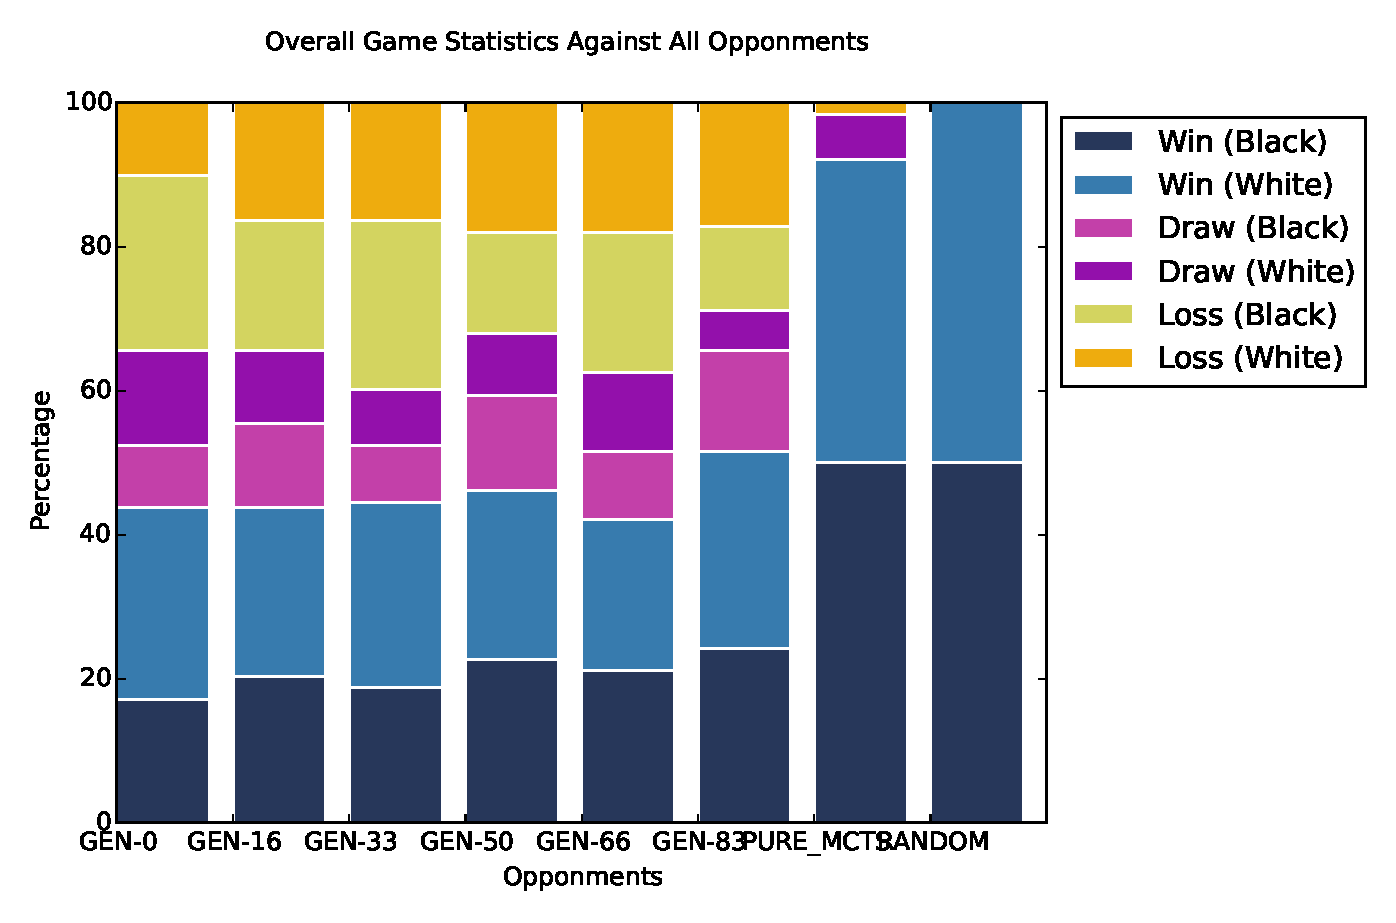
\includegraphics[width=50mm]{images/results/3ply/gm_net_stats.eps}
        %\includegraphics[width=90mm]{images/results/6ply/gm_net_stats.eps}
        \caption{A diagram visualising the crossover process.\label{crossoverpic}}
    \end{figure}
    
        With a ply depth of 3, we can immediately see the impact of the system's performance against other agents that have 
        
    \subsection{Learning Rate}
    % chart of performance over time
    
    The learning rate is derived by comparing a generation's champions with its previous champions from the last five generations. For each older champion, six games are played, with the outcome of the current champion's performance scored and tallied up. An average of the six outcomes are calculated, representing the learning rate. We do not take the learning rate of the first 2 champions due to the lack of available comparisons. This measurement is performed for every generation until the end. It is also the case that this does not influence the actual learning process of the system, but is used as one of the indicators of whether the system is learning in ability over time.
    
    \begin{figure}[!h]
        \centering
        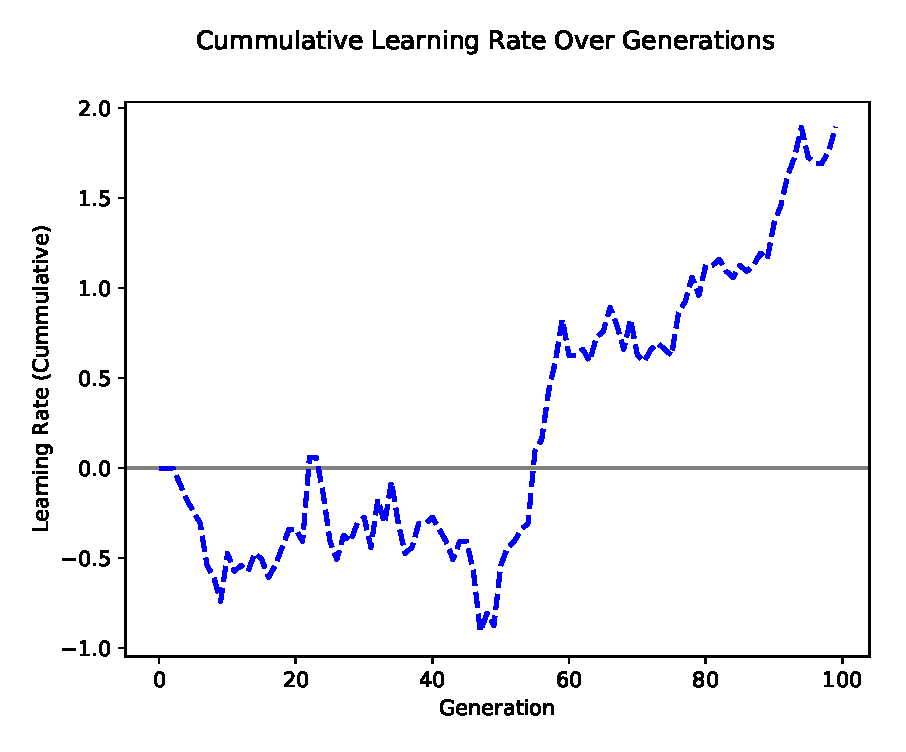
\includegraphics[width=50mm]{images/results/1ply/cummulative_growth.eps}
        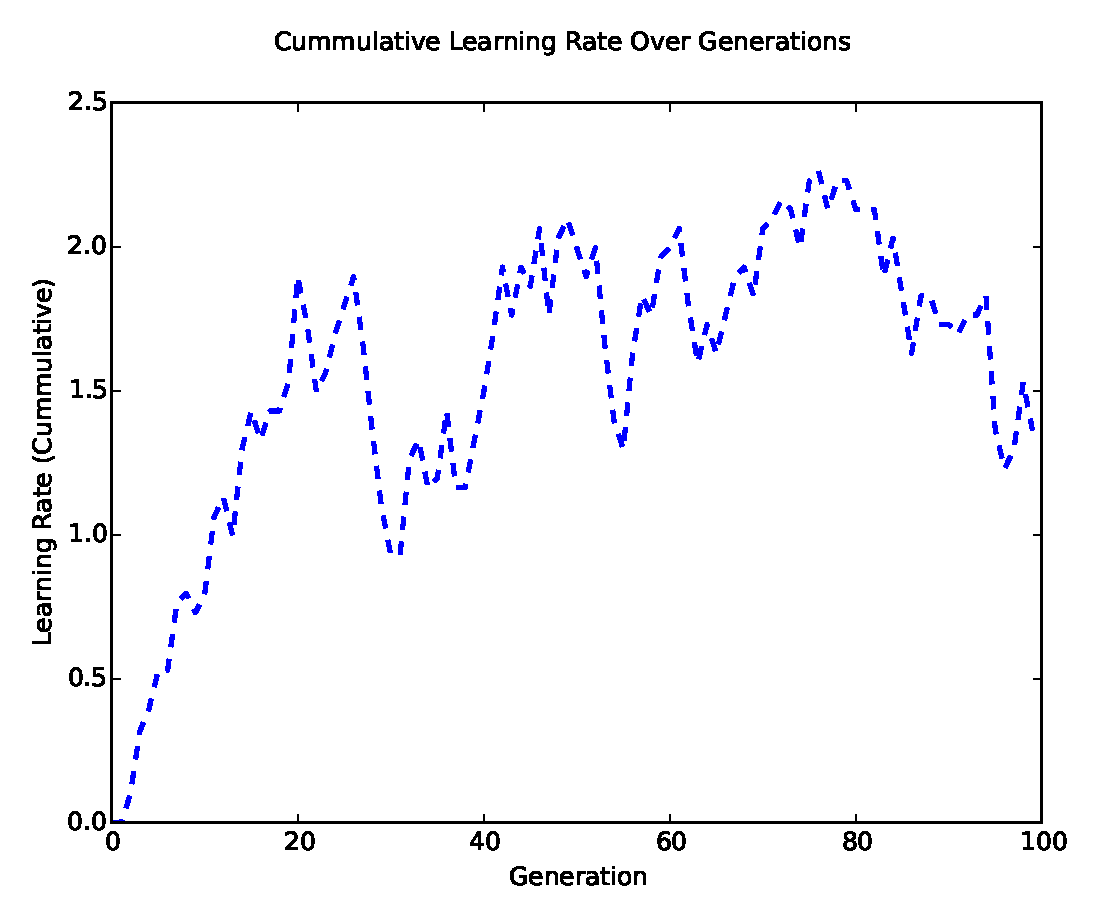
\includegraphics[width=50mm]{images/results/3ply/cummulative_growth.eps}
        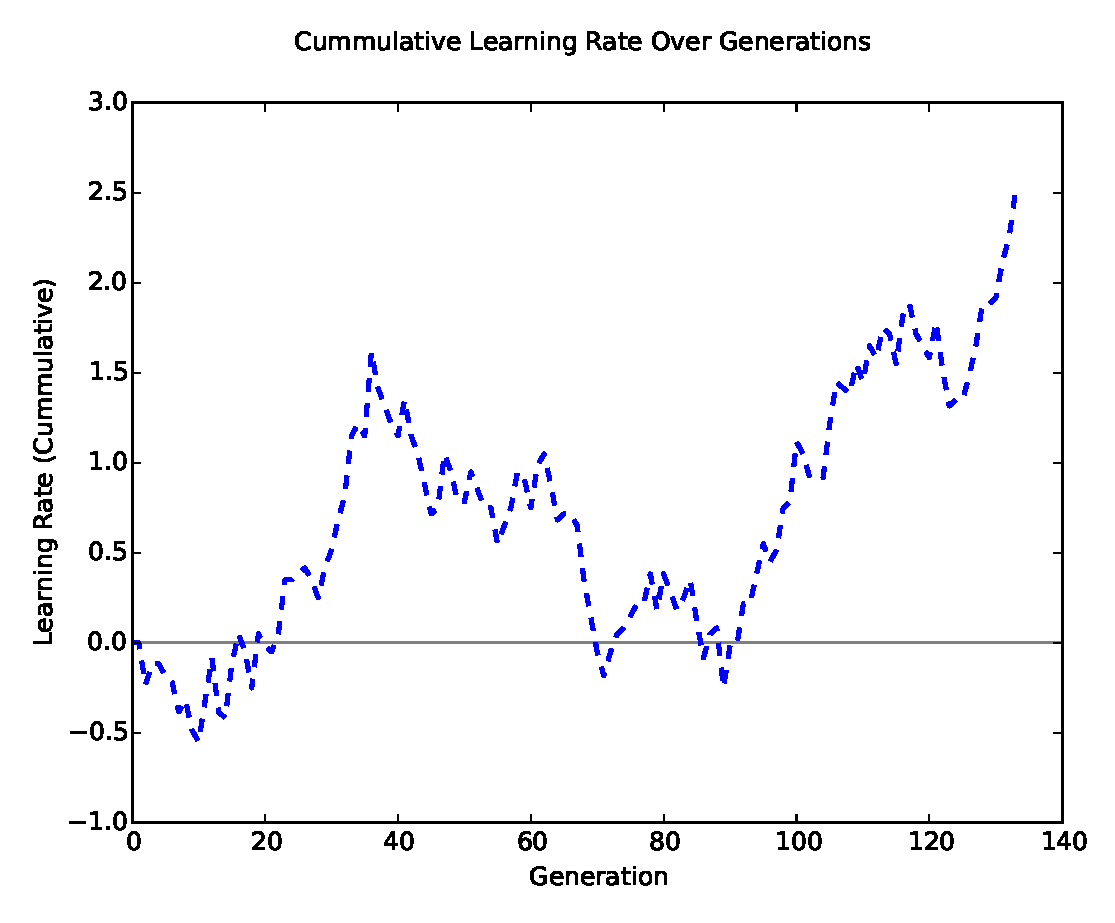
\includegraphics[width=50mm]{images/results/6ply/cummulative_growth.eps}
        \caption{A diagram visualising the crossover process.\label{crossoverpic}}
    \end{figure}
    
    For all ply depths, we can see a cummulative growth such that returns in the net positive as more generations are added. However, even with safe mutations, we can also see that the learning is very volatile. This could relate to our crossover method, where it may be the case that the neural network has implicated a certain heuristic in a different manner to other networks. 
    
    \subsection{Other Observations}
        \subsubsection{Number of Moves}
        \subsubsection{CPU Times}
        \subsubsection{Influence of Inheritance Methods}
    % this section presents the results of the solutions.  It should include information on experimental settings.  The results should demonstrate the claimed benefits/disadvantages of the proposed solutions.
    \subsection{Speed}
    % how fast the system is learning
    
    As predicted, calculating safe mutations is a very computationally expensive endeavour. Efforts to subsidise the performance of 

    % This section should be between 2 to 3 pages in length.





% TODO (WAIT FOR RESULTS)
\section{Evaluation}
% This section should between 1 to 2 pages in length.
    - The quality of the neuroevolutionary algorithm boils down to the quality of the fitness function, which in our case is the tournament; hard to choose the best method
    - Difficult to evaluate moves
    - Naturally slower learning rate than typical ventures as there is an immediate comparision to make against
    - 
    \subsection{Strengths}
    - Fully
    - Without using 
    - Neuroevolution is a viable method for programs with vast search spaces. While this is where both genetic algorithsm can shine. Although this is the case for Deep learning and evolutionary computation in general, the benefit of using genetic algorithms is that the fitness function can be any function, whereas for a neural network, its function needs to be translatable to some form of a differential sum of partial derivatives. 
    - embarrassingly parallel tournaments make it possible to reduce the overall system running time on the system.
    - The system itself relies on a relatively simple learning heuristic that is open to domain specific adaptation.

    
    \subsection{Limitations}
    - creating a high quality fitness function is difficult and its domain specific, or rather, there is no universal fitness function for all problems. This poses as a benefit and a weakness for the neuroevolutionary approach.
        - the fitness function defines the size of the search space and how easily a globally optimal solution can be derived.
        - using a best of champions approach is quite difficult!
        - reality rarely fits into good fitness functions
    - measuring the learning rate is quite difficult and arbitary.
    - compared to other calculus based methods, neuroevolution requires many more samples (often expoentially more) to get a weight of equivalent quality.

    -

    % The challenge with all GA work is finding the right fitness function. If you don't understand your domain well enough to define a good fitness function you're going to be wasting your time, and no amount of algorithmic and/or AI magic is going to help you.
    \subsection{Approach}
    - Should use GPU to improve running times.
    - should have started with times
    Neuroevolution is still in its early stages.
    -If given the chance to repeat the work, we would not change this approach. In hindsight,
having seen that improvements in the clustering field come from new areas, it may have been
better to spend more time in examining references from areas other than computer science,
such as biology and physics, in hope of finding more creative solutions to the clustering
problem.
    - will need to run for longer generations because we can't see a stronger correlation but limited access to high performance computing equipment.

% TODO (WAIT FOR RESULTS)

\section{Conclusions}
    % This section summarises the main points of this paper.  Do not replicate the abstract as the conclusion.  A conclusion might elaborate on the importance of the work or suggest applications and extensions.  This section should be no more than 1 page in length.

    In terms of fufilling its objectives, the project was an overall success. A system was implemented using evolutionary methods and it successfully plays checkers in a manner in which it can learn from over time. To the extent of its growth remains suspect however. Efforts to raise the learning rate is one of the non-trivial challenges that makes neuroevolution a particular field of interest, as it is inherent that it can tackle problems in a somewhat novel manner.
    
    The main findings of this project is as follows:
    - It is evidently possible to create a checkers playing agent that learns to play itself, with little human intervention.
    - some of the the work is 
    - neuroevolution is relatively inefficent compared to their gradient based counterparts. This however forseen due to the heavy dependency of entropy disguised as learning.
    - The fitness function can be anything, but it is important to derive a high quality fitness function.
    
    The major implication is that it is a possible contender for tasks that require unsupervised learning, and that the fitness function cannot be trivially decomposed into set of derivatives that allow regular derivative based learning to shine.
    
    
    There is an incredibly vast scope of future work that would extend the project. One interesting avenue is to consider using a safer method to produce mutation, exercising other contemporary methods in machine learning. 
    Another consideration for the project is to experiment with different crossover algorithms that utilise the temporal difference between inputs and outputs. 
    The quality of the fitness function is especially important.
    promising.


    
% References
\bibliography{zotero}

\end{document}
